# Diagrama de Clases en profundidad

## Repaso: las clases en un D.C.

### Repaso: las clases en un D.C.

\subsubtitleB{Una clase en un diagrama muestra:}

- El nombre de la clase.
- El listado de sus atributos.
    - Indicando su visibilidad.
    - Indicando su tipo de datos.
- El listado de sus operaciones.
    - Indicando su visibilidad.
    - Indicando el tipo de dato de sus parámetros.
        - Opcionalmente el nombre del parámetro.
    - Indicando el tipo de dato que retorna.

\centering\scalebox{0.5}{%
\begin{tikzpicture}
    \umlclass[x=0,y=0]{Vuelo}%
      {--númDeVuelo : Integer\\ --horaSalida : Date\\ --duraciónVuelo : Integer}%
      {+atrasarVuelo(Integer) : Date\\ +obtHoraLlegada() : Date}
    \umlclass[x=8,y=0]{CuentaBancaria}%
      {--dueño : Cliente\\ --balance : Money\\ --apertura : Date}%
      {+depositar(monto : Money) : Boolean\\ +sacar(monto : Money) : Boolean}
\end{tikzpicture}
}

## Repaso: las relaciones en un D.C.

### Repaso: las relaciones en un D.C.

\subsubtitleB{Cardinalidad o multiplicidad}

- Es conveniente detenernos en la cardinalidad.
    - Se usa en varios tipos de relaciones entre clases.

- Valores usados:

\begin{center}
\begin{footnotesize}
\begin{tabular}{cl}
\toprule
\bld{Notación} & \bld{Lectura} \\
\midrule
\bld{1} & Exactamente uno. \\
\bld{n} & Exactamente n. \\
\bld{0..1} & Entre cero y uno. \\
\bld{n..m} & Entre n y m (ambos inclusive). \\
\bld{*} & Cero, uno o cualquier otro número. \\
\bottomrule
\end{tabular} 
\end{footnotesize}
\end{center}


### Repaso: las relaciones en un D.C.

\subsubtitleB{Cardinalidad o multiplicidad}

- Algunas interpretaciones útiles:

\begin{center}
\begin{footnotesize}
\begin{tabular}{cl}
\toprule
\bld{Notación} & \bld{Interpretación} \\
\midrule
Límite inferior \bld{cero} & Es opcional. \\
Límite inferior $\geq$ \bld{uno} & Es obligatorio. \\
\bld{1} & Es ``univaluado''. \\
\bld{*} & Es ``multivaluado'' (implica una lista). \\
\bottomrule
\end{tabular} 
\end{footnotesize}
\end{center}


### Repaso: las relaciones en un D.C.

\subsubtitleB{Asociación}

- Una clase tiene como \bld{propiedad a una instancia de otra clase}.
    - Puede ser una instancia de la misma clase también.
- Se usa una línea continua.
    - Si tiene flecha, indica la \bld{dirección} de la asociación.
- Puede indicarse la \bld{cardinalidad} de la asociación.
- Suele indicarse el nombre que la propiedad tiene en la clase ``contenedora''.

\begin{center}
\scalebox{0.5}{%
\begin{tikzpicture}
    \umlclass[x=0,y=0]{Orden}
        {--fecha : Integer\\--prepagada : Boolean}
        {+enviaEmail() : Boolean}
    \umlclass[x=10,y=0]{Cliente}
        {--nombre : String\\--dirección : String\\--antigüedad : Integer}
        {}
    \umluniassoc[mult1=*,pos1=0.1,mult2=1,arg2=Emisor,pos2=0.85]{Orden}{Cliente}
\end{tikzpicture}
}
\end{center}

### Repaso: las relaciones en un D.C.

\subsubtitleB{Dirección en una asociación}

Fundamentalmente tenemos dos casos:

- Ambas clases son ``conscientes'' de la asociación: \bld{bi-direccional}.

\begin{center}
\scalebox{0.5}{%
\begin{tikzpicture}
    \umlclass[x=0,y=0]{Persona}
        {--nombre : String\\--edad : Integer\\--sexo : Char}
        {}
    \umlclass[x=10,y=0]{Automóvil}
        {--color : String\\--marca : String\\--año : Integer}
        {}
    \umlbiassoc[mult1=0..1,arg1=dueño,pos1=0.15,mult2=*,pos2=0.85]{Persona}{Automóvil}
\end{tikzpicture}
}
\end{center}

- Implica algún mecanismo de ``sincronización''.
- Se diagrama \bld{con dos flechas}, o también \bld{con ninguna}.

### Repaso: las relaciones en un D.C.

\subsubtitleB{Dirección en una asociación}

En este caso de \bld{asociación bi-direccional}:

\begin{center}
\scalebox{0.5}{%
\begin{tikzpicture}
    \umlclass[x=0,y=0]{Persona}
        {--nombre : String\\--edad : Integer\\--sexo : Char}
        {}
    \umlclass[x=10,y=0]{Automóvil}
        {--color : String\\--marca : String\\--año : Integer}
        {}
    \umlbiassoc[mult1=0..1,arg1=dueño,pos1=0.15,mult2=*,pos2=0.85]{Persona}{Automóvil}
\end{tikzpicture}
}
\end{center}

- Una persona puede tener ninguno, uno o muchos automóviles.
    - Entre sus atributos habrá una lista de automóviles.
- Un automóvil tiene un solo dueño, o puede no tener ninguno aún.
    - Tendrá un atributo llamado \bld{dueño}, pues así está indicado en el diagrama.

### Repaso: las relaciones en un D.C.

\subsubtitleB{Dirección en una asociación}

Fundamentalmente tenemos dos casos:

- Sólo una clase es ``consciente'' de esta relación: \bld{uni-direccional}.

\begin{center}
\scalebox{0.5}{%
\begin{tikzpicture}
    \umlclass[x=0,y=0]{ReporteCuentasSobregiradas}
        {--fechaGeneración : Date}
        {+actualizar() : Boolean}
    \umlclass[x=10,y=0]{CuentaBancaria}%
      {--balance : Money\\ --apertura : Date}%
      {+depositar(monto : Money) : Boolean\\ +sacar(monto : Money) : Boolean}
    \umlclass[x=10,y=-5]{Cliente}
        {--nombre : String\\--dirección : String\\--antigüedad : Integer}
        {}
    \umluniassoc[mult2=*,arg2=ctasSobreg,pos2=0.7]{ReporteCuentasSobregiradas}{CuentaBancaria}
    \umlbiassoc[mult1=0..1,arg1=dueño,pos1=0.2,mult2=*,pos2=0.8]{Cliente}{CuentaBancaria}
\end{tikzpicture}
}
\end{center}

### Repaso: las relaciones en un D.C.

\subsubtitleB{Dirección en una asociación}

En este caso de \bld{asociación uni-direccional}:

\begin{center}
\scalebox{0.5}{%
\begin{tikzpicture}
    \umlclass[x=0,y=0]{ReporteCuentasSobregiradas}
        {--fechaGeneración : Date}
        {+actualizar() : Boolean}
    \umlclass[x=10,y=0]{CuentaBancaria}%
      {--dueño: Cliente\\ --balance : Money\\ --apertura : Date}%
      {+depositar(monto : Money) : Boolean\\ +sacar(monto : Money) : Boolean}
    \umluniassoc[mult2=*,arg2=ctasSobreg,pos2=0.7]{ReporteCuentasSobregiradas}{CuentaBancaria}
\end{tikzpicture}
}
\end{center}

- Los reportes tienen un listado de las cuentas involucradas.
- Las cuentas no tienen forma de entregar el o los reportes donde son mencionadas.
    - Esto es claramente una decisión de diseño.
    - Permite aliviar el modelo de restricciones de sincronización.
        - Se hace en los casos en que no es tan relevante que una clase sepa que ``están
        hablando de ella en otra parte''.

### Repaso: las relaciones en un D.C.

\subsubtitleB{Asociaciones reflexivas}

- Una instancia de una clase puede perfectamente tener como atributo una instancia distinta de ella misma.

\begin{center}
\scalebox{0.6}{%
\begin{tikzpicture}
    \umlclass[x=0,y=0]{Persona}
        {--nombre : String\\--edad : Integer\\--sexo : Char}
        {}
    \umluniassoc[mult1=1,arg1=padre,pos1=0.1,angle1=-90,angle2=-180,loopsize=40mm,mult2=*,pos2=0.9,arg2=hijo]{Persona}{Persona}
\end{tikzpicture}
}
\end{center}

### Repaso: las relaciones en un D.C.

\subsubtitleB{Clases de asociación}

- Hay veces que una asociación puede tener atributos en sí misma.
- En algunos casos, conviene encapsular esos atributos en una nueva clase.


\begin{center}
\scalebox{0.5}{%
\begin{tikzpicture}
    \umlclass[x=0,y=0,width=10em]{Cliente}
        {--nombre : String\\--dirección : String\\--antigüedad : Integer}
        {}
    \umlclass[x=10,y=0,width=10em]{Automóvil}
        {--color : String\\--marca : String\\--año : Integer}
        {}
    \umlbiassoc[name=assoc,mult1=0..1,pos1=0.15,mult2=*,pos2=0.85]{Cliente}{Automóvil}
    \umlassocclass[x=5,y=-4,width=10em]{Arriendo}{assoc-1}{--fechaIni : Date\\ --fechaFin : Date\\ --precio : Money}{}
\end{tikzpicture}
}
\end{center}

- Ojo con la línea segmentada.

### Repaso: las relaciones en un D.C.

\subsubtitleB{Herencia}

\begin{description}
    \item[Generalización:] Se tiene cuando dadas dos o más clases con características y/o comportamiento en común:
    \begin{itemize}
        \item Modelamos una nueva clase que refleje aquello que ellas comparten.
    \end{itemize}
\vfill
    \item[Especialización:] Cuando una clase está comprendiendo muchas características, no siempre presentes en sus instancias:
    \begin{itemize}
        \item Modelamos varias clases, donde cada una se encarga de esas características específicas.
        \item Las clases producidas deben tener sentido en nuestro modelo.
    \end{itemize}
\end{description}

### Repaso: las relaciones en un D.C.

\subsubtitleB{Herencia}

Por ejemplo:

- Nuestra aplicación bancaria maneja muchos datos de clientes y de avales.
    - Vemos que sus características son prácticamente las mismas.
    - Muchos de sus comportamientos son iguales.
    - Generamos una generalización llamada... \bld{Persona}.

\centering\scalebox{0.6}{%
\begin{tikzpicture}
    \umlclass[x=0,y=0]{Persona}{}{}
    \umlclass[x=-2,y=-3]{Cliente}{}{}
    \umlclass[x=2,y=-3]{Aval}{}{}
    \umlinherit{Cliente}{Persona}
    \umlinherit{Aval}{Persona}
    % \umlrelation[style={tikzuml inherit style}]{Cliente}{Persona}
\end{tikzpicture}
}

### Repaso: las relaciones en un D.C.

\subsubtitleB{Herencia}

Por ejemplo:

- Nuestra aplicación maneja información de los empleados en una empresa (quizás es un ERP).
    - Comenzamos pensando en los empleados en general.
    - Pronto nos damos cuenta que no todas las características ni comportamientos aplican
    a todos por igual.
    - Hay cosas que son específicas: creamos las clases \bld{Gerente} y \bld{Vendedor}.

\centering\scalebox{0.6}{%
\begin{tikzpicture}
    \umlclass[x=0,y=0]{Empleado}{}{}
    \umlclass[x=-2,y=-3]{Gerente}{}{}
    \umlclass[x=2,y=-3]{Vendedor}{}{}
    \umlinherit{Gerente}{Empleado}
    \umlinherit{Vendedor}{Empleado}
\end{tikzpicture}
}

## Miembros estáticos

### Miembros estáticos

\subsubtitleB{Atributos, hasta ahora:}

- Ya hemos visto que las clases pueden tener atributos.
    - Los valores de los atributos son propios de cada instancia (objeto) creado.
        - La clase \texthigh{Aeroplano} posee el atributo \texthigh{color}.
        - Una instancia puede ser de color \textcolor{orange}{naranja}.
        - Otra instancia puede ser de color \textcolor{gray}{gris}.
        - Otra instancia puede ser de color \textcolor{green}{verde}.

\vfill

\columnsbegin
\column{0.33\textwidth}
\centering
\includegraphics[width=20mm]{icons/92-emoji_android_airplane.png}
\column{0.33\textwidth}
\centering
\includegraphics[width=20mm]{icons/92-emoji_android_airplane_gray.png}
\column{0.33\textwidth}
\centering
\includegraphics[width=20mm]{icons/92-emoji_android_airplane_green.png}
\columnsend

### Miembros estáticos

\subsubtitleB{Atributos estáticos:}

- Una clase puede definir algunos atributos como \bld{\texthigh{estáticos}}:

\buildrboxx[0.9\textwidth]{}

- Todas sus instancias tienen este atributo.
- Pero todas ellas \texthigh{comparten el mismo valor} de este atributo.
    - Si una de ellas lo cambia, las demás también lo verán cambiado.

\finishrboxx

- Se les llama también \texthigh{atributos de clase}.

### Miembros estáticos

\subsubtitleB{Operaciones, hasta ahora:}

- Para el caso de las operaciones, sabemos que todas las instancias de una clase
tienen a su disposición las operaciones de esa clase.
    - Todos los aeroplanos pueden volar.
        - Dependiendo de su ubicación y velocidad actual, cada aeroplano volará en cada instante
        ``a su propia manera''.
    - Todos los aeroplanos puede entregar su cantidad actual de pasajeros.
        - Cada instancia entregará un número en particular.

\vfill

\columnsbegin
\column{0.33\textwidth}
\centering
\includegraphics[width=20mm]{icons/92-emoji_android_airplane_withpeople.png}
\column{0.33\textwidth}
\centering
\includegraphics[width=20mm]{icons/92-emoji_android_airplane_gray_withpeople.png}
\column{0.33\textwidth}
\centering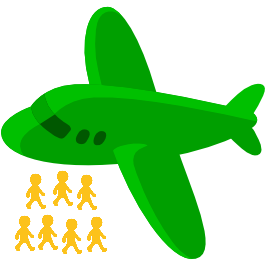
\includegraphics[width=20mm]{icons/92-emoji_android_airplane_green_withpeople.png}
\columnsend

### Miembros estáticos

\subsubtitleB{Operaciones estáticas:}

- Una clase puede definir algunas operaciones como \bld{\texthigh{estáticas}}:

\buildrboxx[0.9\textwidth]{}

- Las instancias \texthigh{no tienen acceso} a esa operación.
- Pasa a ser una operación \texthigh{propia de la clase}.
- El resultado ---y la manera de obtenerlo--- no dependen de las particularidades de ninguna instancia de la clase.

\finishrboxx

### Miembros estáticos

\subsubtitleB{Operaciones estáticas:}

- Hay clases que definen casi todas sus operaciones como estáticas:
    - En Java, la clase \texttt{Math} provee funciones matemáticas.
    - Calcular la tangente de un ángulo, o determinar el menor entre dos números, no son
    operaciones que dependan de alguna circunstancia en particular.
        - No existen ``distintas versiones de la matemática'' que las implementen de manera
        diferenciada.

### Interfaces

TODO:

\subsubtitleB{}


### Relación entre D.C. y D.S.

Entre los diagramas de clases y de secuencia tenemos:

- Ya sabemos que los objetos no son entes estáticos.
    - No solamente guardan datos o propiedades de cada instancia.
    - También \bld{interactúan} entre sí o con instancias de otras clases.

- La interacción se lleva a cabo a través de \alert{mensajes}.
    - Una instancia, al recibir un mensaje, la procesa mediante una operación (implementada en
    un método).
    - Al conjunto de mensajes que una instancia pueda antender, se le denomina \alert{interfaz}.
        - \bld{Ojo} con los distintos usos de la palabra interfaz.
